\setlength{\headheight}{13.59999pt}

\note{come back to this after sections are written}

This chapter is concerned with the method we have used to create semi-analytic models of planet wakes that encompass both the linear and non-linear disk response due to a perturbing planet as described in the previous chapter. 
This work builds on that presented in \citet{bollati2021} and so we will be predominantly concerned with the differences from their analysis.
However we aim to provide enough detail to be understandable without having read the aforementioned paper.

\section{Wakeflow: A Python Package For Semi-Analytic Models of Planet Wakes} \label{sec:JOSS}

This section has been submitted to the Journal of Open Source Science and is currently in review. The preprint is publicly available here: \url{https://github.com/TomHilder/wakeflow/blob/master/paper/paper.md}

\subsubsection{Summary}

\textsc{wakeflow} is a Python package for generating semi-analytic models of the perturbations induced by planets embedded in gaseous circumstellar disks. 
These perturbations take the form of a spiral shock wave \citep{ogilvie2002}, and are often called a ``planet wake'' in analogy with that produced by a boat in a lake.

\subsubsection{Statement of Need}

Detecting newly formed planets embedded in their disk is a challenging problem in the field of planet formation. 
A major area of progress in recent years is the detection of planets by the gravitationally induced disturbance in their host disks. 
This disturbance, caused by the planet wake, manifests as a deviation in velocity from the bulk flow which may be measured through the Doppler shift of molecular lines \citep[eg.][]{perez2015, pinte2018a}. 
Such kinematic observations have been accurately reproduced through 3D fluid simulations of the planet-disk interaction, allowing for the inference of planet and disk properties \citep{pinte2018a, pinte2019}. 
However, these studies are computationally expensive.

\textsc{wakeflow} eases this computational cost by applying the theory of planet wake generation and propagation \citep{goldreich1979,goodman2001,rafikov2002a,bollati2021} to create semi-analytic models of planet wakes. 
\textsc{wakeflow} models are readily created in a few seconds on a modern laptop, as opposed to the hours of supercomputer time needed for 3D hydrodynamical simulations. 
The relatively low computational cost of \textsc{wakeflow} means that researchers can get an idea of whether planet-disk interactions can explain their observations, and the disk and planet parameters needed, before spending computer time on more detailed simulations.

\textsc{wakeflow} can interface with the radiative transfer code \textsc{mcfost} \citep{pinte2006,pinte2009} in order to create synthetic observations of the semi-analytic models for direct comparison with observed continuum or line emission.

\textsc{wakeflow} is partially adapted from a previous Python code also written by us called \textsc{analytical\_kinks} \citep{bollati2021a}. 
\textsc{wakeflow} is intended to be a more complete, versatile and easy to use version of that code, and it obeys standard Python packaging conventions.
In addition, \textsc{wakeflow} can directly interface with \textsc{mcfost} while \textsc{analytical\_kinks} cannot.
At the time of writing, no other open source software packages exist to generate the perturbations induced by an embedded planet in a circumstellar disk using the semi-analytic theory of planet wakes.

Existing scientific publications focusing on detecting the kinematic signatures of planets that have used \textsc{wakeflow} or its predecessor \textsc{analytical\_kinks} include \citet{bollati2021}, \citet{calcino2022}, \citet{teague2022}, \citet{garg2022} and \citeauthor{fasanoinprep.} (in prep.).

\subsubsection{Acknowledgements}

\textsc{wakeflow} relies on the following scientific Python packages: \textsc{NumPy} \citep{harris2020}, \textsc{matplotlib} \citep{hunter2007}, \textsc{SciPy} \citep{virtanen2020} and \textsc{Astropy} \citep{astropycollaboration2022}.

\section{Semi-Analytic Solution Algorithm}

\begin{figure}
    \centering
    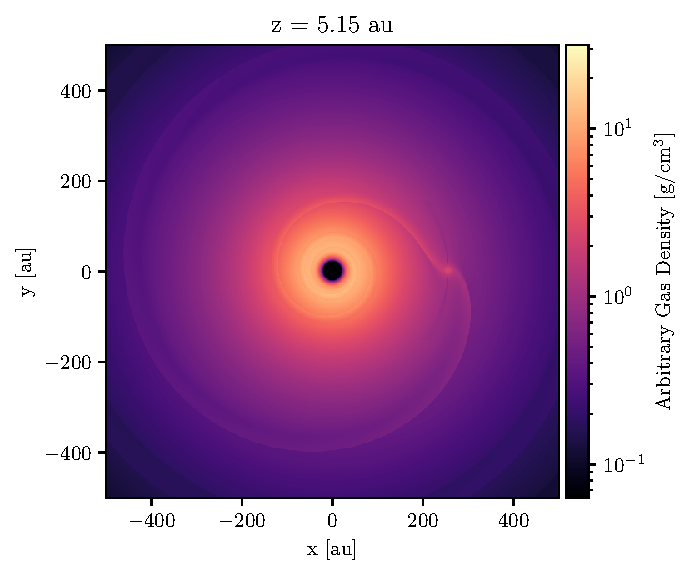
\includegraphics[width = 0.85\textwidth]{figures/wakeflow_tutorial_plot.pdf}
    \caption{Density slice of a \textsc{wakeflow} model at constant height $z=5.15$ au, plotted with a logarithmic colourbar. The model contains a $0.5 \, M_{\rm J}$ planet, placed at a separation of $256$ au from the central star. These results were generated following the quickstart tutorial publicly available on the \textsc{wakeflow} documentation\protect\footnotemark[4], and are meant as a model of the planet wake in the disk of HD 163296, with disk parameters chosen following \citet{pinte2018a} and \citet{calcino2022}.}
    \label{fig:example_model}
\end{figure}

\footnotetext[4]{\url{https://wakeflow.readthedocs.io/en/latest/tutorials/quickstart.html}}

Here we provide an overview of the algorithm used by \textsc{wakeflow} to generate models.
For stages that are sufficiently different to \citet{bollati2021}, further detail will be provided in the section \ref{sec:model_considerations}.
The algorithm proceeds as:
\begin{enumerate}
    \item The global grid geometry is generated based on the user's choice of grid geometry and number of grid points. Both cylindrical and cartesian grid geometries are supported, as well as the \textsc{mcfost} grid geometry if the user wishes to generate synthetic observations from their model.
    
    The run time for \textsc{wakeflow} scales linearly in the number of grid points $n_x \times n_y$ or $n_r \times n_\phi$, but is roughly independent of the number of points in the vertical direction $n_z$..
    
    \item The unperturbed disk density and velocity structure is calculated based on the user's choice of disk parameters as outlined in section \ref{sec:diskstruct}.
    
    \item The linear perturbations are calculated and mapped onto the global disk geometry, following section \ref{sec:linear_box}. The perturbations $\sigma, u$ and $v$ are assumed to be independent of vertical height $z$.
    
    \item The initial conditions for the non-linear evolution are extracted from the edge of the linear regime along a slice of constant $t$, as described in \ref{sec:transformations}.
    
    \item Burger's equation is solved in $(t,\eta)$ space until $t_{\rm f}=300$ using a vectorised Godunov solver \citep{astrofluids}. Unlike in \citet{bollati2021} we use make use of adaptive time-steps, which both ensures the stability of the solution (especially for large planet masses that shock quickly), as well as improves efficiency as large time-steps are taken when appropriate. After $t_{\rm f}$, the asymptotic solution is taken as described in \citet{bollati2021}.
    
    \item The solution $\chi(t,\eta)$ is transformed to $\chi(r,\phi)$ as described in section \ref{sec:transformations}.
    
    \item The density perturbations in the non-linear regime are calculated from $\chi$ using equations \ref{eq:chi} and \ref{eq:g_power}. The velocity perturbations are calculated from $\chi$ as described in section \ref{sec:velocity_perts}. Again, all perturbations $\sigma, u$ and $v$ are assumed to be independent of $z$.
    
    \item The results are written to the disk. This output may be a \textit{.fits} file if desired.
\end{enumerate}

\noindent A density slice of an example \textsc{wakeflow} model is shown in Figure \ref{fig:example_model}.
This model was calculated on a $1000 \times 1000 \times 30$ grid in $x,y$ and $z$ respectively, and took in $19.1$ seconds to compute on an Apple M1 processor.

\section{Theoretical and Numerical Considerations} \label{sec:model_considerations}

\note{Add something about how we are basically going into more detail for the steps in the algorithm and explaining the specific applications of or improvements to the stuff that been done before.}

\subsection{Unperturbed Disk Structure} \label{sec:diskstruct}

Here we outline the unperturbed disk model used in \textsc{wakeflow} onto which the perturbations are added.

\subsubsection{Temperature}

We assume that the sound speed $c$ obeys a simple radial power law 
\begin{align}
    c \propto r^{-q},
\end{align}
where $q$ is some real number. Thus the disk temperature scales as 
\begin{align}
    T \propto c^2 \propto r^{-2q}.
\end{align}
The constant of proportionality for these relations in determined by the user specified value of the disk aspect ratio $H/r$ at $r=r_{\rm ref}$

\subsubsection{Density}

We use a density structure derived by assuming that the disk is in vertical hydrostatic equilibrium \citep{pringle1981}, but unlike in \ref{eq:vertical_rho} we will not assume that $z\ll r$.
The density $\rho$ is given by 
\begin{align}
    \rho(r,z) \propto \left( \frac{r}{r_{\rm ref}} \right)^{-p} \exp{\left( \frac{G M_\star}{c^2} \left[ \frac{1}{\sqrt{r^2 + z^2}} - \frac{1}{r} \right] \right)},
\end{align}
where $p$ is some real number. 
The constant of proportionality is set directly by the user, or calculated by \textsc{mcfost} based on the total gas mass.

Very commonly the density profile is parameterised in terms of the surface density $\Sigma$, not the actual density $\rho$ as above.
If the surface density is parameterised as $\Sigma \propto r^{-\delta}$ where $\delta$ is some real number, then equation \ref{eq:surf_dens_to_dens} gives the approximate relation 
\begin{align}
    p \simeq \frac{3}{2} - q + \delta,
\end{align}
which can be used to convert between density parameterisations.
This conversion is only approximate in our context, since is does assume that $z \ll r$ and our density profile does not.
However this turns out not to matter since $\delta$ will only show up in the $t(r)$ mapping which we will assume is the same for all $z$.

\subsubsection{Velocities}

The radial and vertical motions in the unperturbed disk are set to zero. 
The rotation is derived assuming radial force balance \citep[eg.][]{nelson2013} and is given by 
\begin{align}
    \Omega(r,z) = \Omega_{\rm K} \left[ - \left(p + 2q\right) \left( \frac{H}{r} \right)^2 + \left( 1-2q \right) + \frac{2qr}{\sqrt{r^2 + z^2}}\right]^{1/2},
\end{align}
where $\Omega_{\rm K}$ is as defined in equation \ref{eq:point_pot}.

\subsection{Linear Box} \label{sec:linear_box}

The solution in the linear regime nearby the planet used in \textsc{wakeflow} was calculated by \citet{bollati2020} and \citet{bollati2021} by solving equations \ref{eq:fourier_v} -- \ref{eq:fourier_sigma} numerically following the procedure outlined in \citet{goodman2001}.
Here, we simply read their dimensionless calculations and scale them accordingly for our purposes. Figure \ref{fig:lin_box_bollati} shows the $u$ and $v$ solutions presented in \citet{bollati2021} in local cartesian coordinates $x,y$ centred on the planet location.
The $x,y$ coordinates are scaled by the Mach-1 length $l_{\rm p} = 2H_{\rm p}/3$, while the perturbation are scaled by the planet mass in units of the thermal mass $M_{\rm p} / M_{\rm th}$.

\begin{figure}
    \centering
    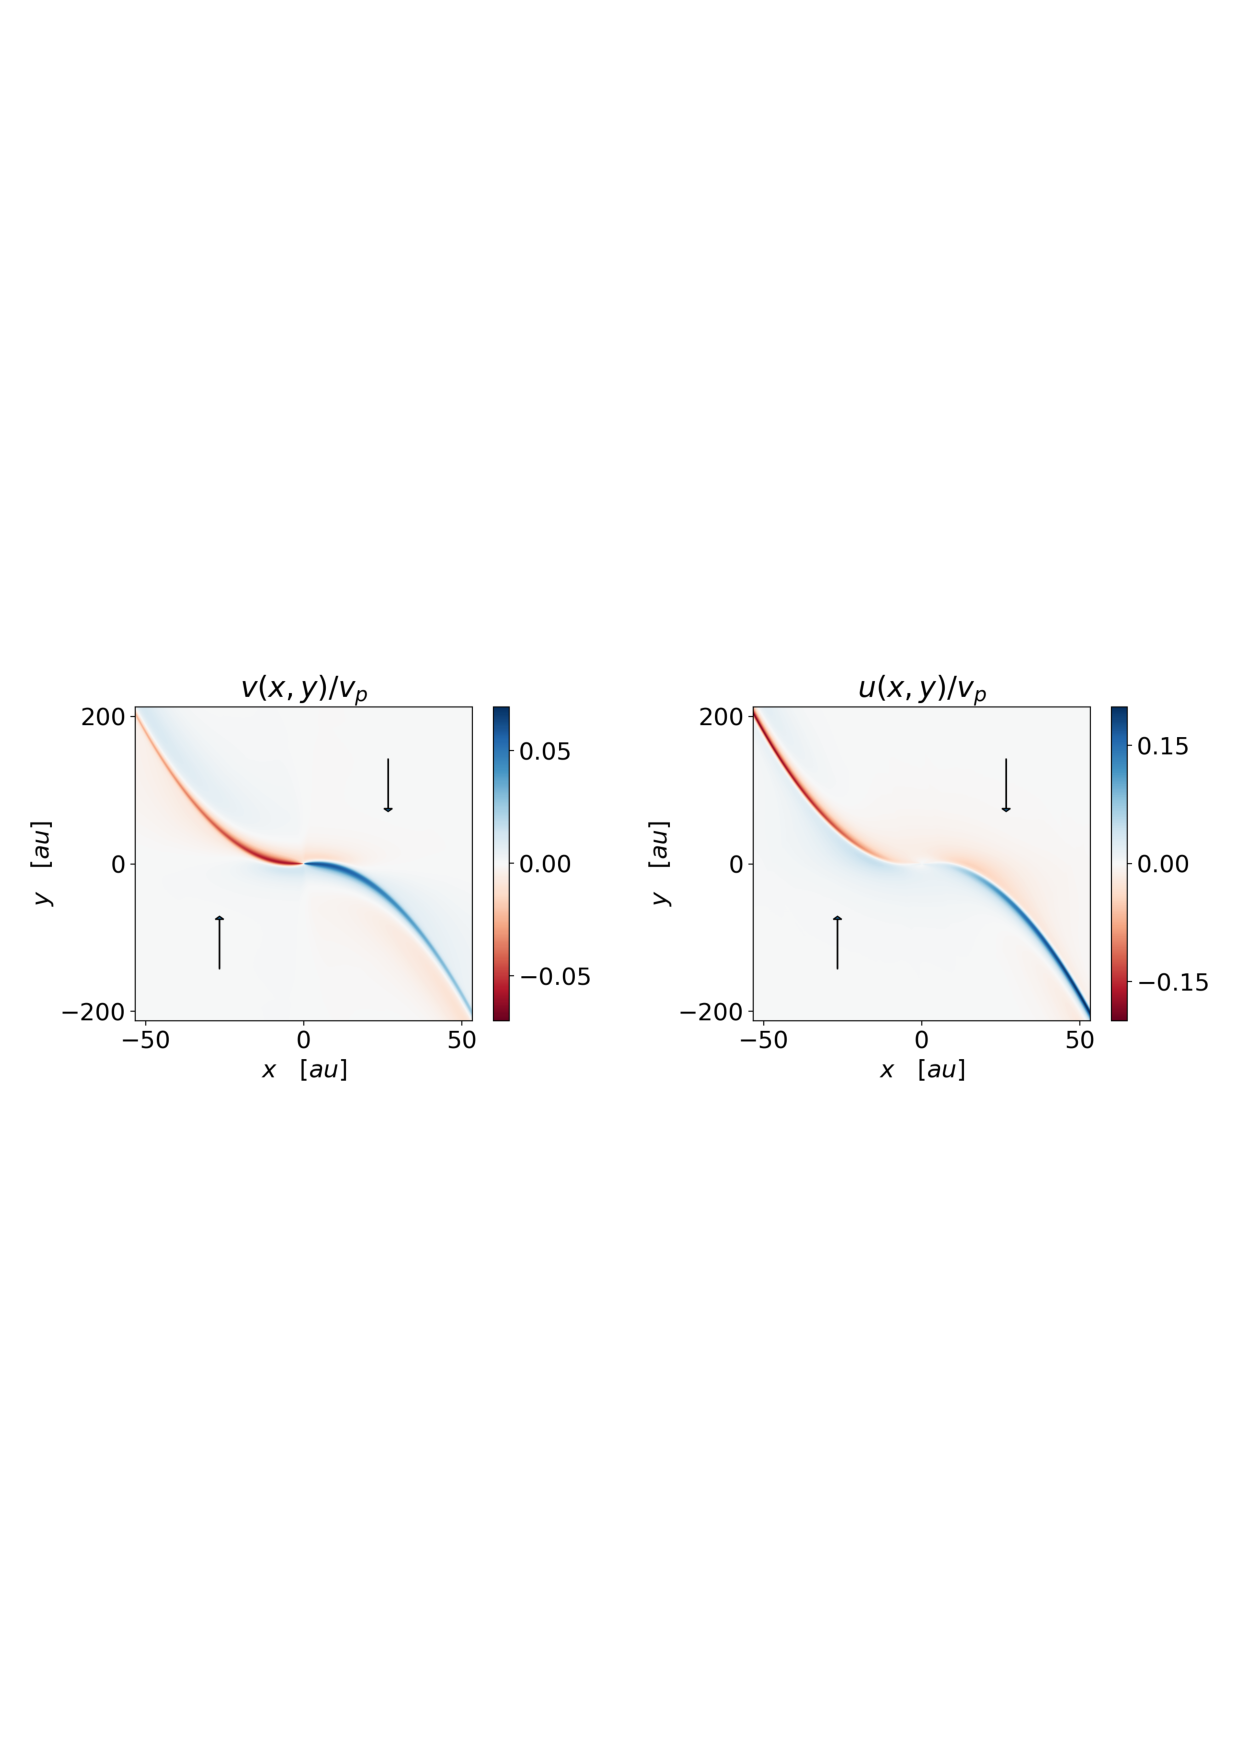
\includegraphics[width = 0.95\textwidth]{figures/linear_box_bollati.pdf}
    \caption{Linear azimuthal (left) and radial (right) velocity perturbations $v$ and $u$ centred on the planet in local cartesian coordinates as defined in equations \ref{eq:local_x} and \ref{eq:local_y}, and calculated by \citet{bollati2021}. The velocity is given in units of $v_{\rm p} = \Omega_{\rm K}(r_{\rm p})$, and the arrows denote the direction of the shearing bulk gas flow in a frame centred on the planet.}
    \label{fig:lin_box_bollati}
\end{figure}

Unlike \citet{bollati2021}, we do not include the linear regime results as a square box in the global solution.
Instead, we take seriously the transformation \ref{eq:local_y}, and interpret $y$ as an arc-length instead of a true Cartesian coordinate, giving us a \textit{linear annulus segment} instead of a \textit{linear square box} (we will from now on refer to the former simply as the \textit{linear box}).
Indeed, when the $\chi$ initial condition is extracted from the edge of the box, this is the treatment used for $y$.
It is therefore more honest to take this approach when mapping the linear solution onto the global grid, and has the added benefit of resulting in a more continuous solution.
In addition, we allow for separate variation of the height (angular extent) and width (radial extent) of the box.
This is motivated by considering that the box size was originally chosen as the Mach-1 length through an argument about resonance location (see section \ref{sec:linear_wake_excitation}).
Since these locations are constant as $\phi$ varies, it is perfectly acceptable to extent the linear regime in the angular direction.
The caveat to this is that the linear solution was derived in the shearing sheet approximation where the global geometry of the disk is not considered.
The curvature of the $y$ coordinate becomes more extreme as the box size increases angularly.

\subsection{Transformations} \label{sec:transformations}

To perform transformation between the physical coordinates and $(t,\eta)$ space in calculating our models, we apply the general forms of the transformations \ref{eq:g} -- \ref{eq:eta} to so-called \textit{power-law disks} where the sound speed and surface density are parameterised as
\begin{align}
    c(r) = c_{\rm p} \left(\frac{r}{r_{\rm p}}\right)^{-q}; \quad \Sigma(r) = \Sigma_{\rm p} \left(\frac{r}{r_{\rm p}}\right)^{-\delta},
\end{align}
where $c_{\rm p}$ and $\Sigma_{\rm p}$ are the sound speed and surface density at $r_{\rm p}$.
Assuming also that $\Omega=\Omega_{\rm K}$, then equation \ref{eq:phi_wake} becomes \citep{rafikov2002a}
\begin{align}
    \phi_{\rm wake}(r) = \phi_{\rm p} + {\rm sgn} \left( r - r_{\rm p} \right) \frac{r_{\rm p}}{H_{\rm p}} \left[ \frac{2}{2q-1} \left(\frac{r}{r_{\rm p}}\right)^{q-\frac{1}{2}} - \frac{1}{q+1} \left(\frac{r}{r_{\rm p}}\right)^{q+1} - \frac{3}{\left(2q-1\right)\left(q+1\right)} \right].
\end{align}
Additionally, the Keplerian rotation implies $|2A| = 3\Omega/2 = 3c/2H$ and so the Mach-1 length becomes
\begin{align}
    l_{\rm p} = \frac{2H}{3},
\end{align}
and so the $\eta$ transformation \ref{eq:eta} reduces to 
\begin{align}
    \eta(r, \phi) = \frac{3 r_{\rm p}}{2 H_{\rm p}} \left[ \phi - \phi_{\rm wake} \right].
\end{align}
Additionally the $t$ transformation becomes \citep{rafikov2002a}
\begin{align}
    t(r) = \frac{3}{2^{5/4}} \left( \frac{r_{\rm p}}{H_{\rm p}} \right)^{\frac{5}{2}} \left| \int_1^{r/r_{\rm p}} |s^\frac{3}{2} - 1|^\frac{3}{2} s^{\frac{5q+\delta}{2}-\frac{11}{4}}\, ds \right|, \label{eq:t_power}
\end{align}
where explicitly the $g$ function is given by \citep{bollati2021}
\begin{align}
    g(r) = 2^{1/4} \left( \frac{r_{\rm p}}{H_{\rm p}} \right)^{\frac{1}{2}} \frac{\left( \frac{r}{r_{\rm p}} \right)^{\frac{5}{4} - \frac{\delta + 3q}{2}}}{\left| 1 - \left(\frac{r}{r_{\rm p}}\right)^\frac{3}{2} \right|^\frac{1}{2}} \label{eq:g_power}
\end{align}
This gives us all the tools we need to map from $(r,\phi)$ space to $(t,\eta)$ space in a Keplerian power law disk.
These are the forms of the transformations used by \textsc{wakeflow}.
We are therefore implicitly assuming that the unperturbed rotation profile is well approximated as Keplerian in the mid-plane, which is reasonable since the correction is of order $\left(H/r\right)^2$.

Unlike in \citet{goodman2001,rafikov2002a,bollati2021} we do not use approximate forms of the transformations that hold nearby the planet in the shearing sheet approximation to extract the initial condition for the Burger's evolution.
We found that the approximate transformation for $\eta$ \citep[equations 35 in][]{rafikov2002a} shifted the wake profile in $\eta$ by a few percent, leading to a discontinuity in the solution at the interface between the linear and non-linear regimes.
The approximate $t$ transformation has a similar effect although it is much smaller.
For this reason we always use the exact transformations as listed above.

Previously \citet{bollati2021} assumed that the initial condition for the inner ($r<r_{\rm p}$) and outer ($r>r_{\rm p}$) wake propagation were identical and so solved only the outer wake case and copied the solution for the inner wake.
This approximation does not hold well except for very small values of $(H/r)_{\rm p}$, as the radial extent of the box results in different $t$ coordinates at the inner and outer edge of the box in general.
For this reason we instead solve separately the inner and outer wake propagation, taking the appropriate initial condition for each (\citeauthor{fasanoinprep.}, in prep.).

After Burger's equation is solved numerically, the solution must be mapped from $\chi(t,\eta)$ to $\chi(r,\phi)$.
Since $t(r)$ is not invertible, we instead find the $(t,\eta)$ coordinates of every point on the solution grid $(r,\phi)$ and interpolate from the Burger's solution in $t,\eta$ space.
We therefore must evaluate the $t(r)$ and $\eta(r,\phi)$ transformations $N$ times, where $N$ is the number of points in the grid.
The $\eta$ transformation is easily vectorised since it is a simply algebraic expression, however the $t(r)$ transformation \ref{eq:t_power} involves an integral which naively must be evaluated $N$ times.
This approach is very inefficient, since the integral in the transformation does not actually depend on $r$, merely the end point does.
Re-evaluating the integral each time therefore often involves integrating over the same interval very many times.
In \textsc{wakeflow} we instead convert mapping $r\rightarrow t$ into an initial value problem (IVP).
Since the integrands of equation \ref{eq:t} is independent of r, we can convert equation \ref{eq:t} into an ordinary differential equation with an appropriate initial condition
\begin{align}
    \frac{dt(s)}{ds} = \frac{r_{\rm p}}{l_{\rm p}} \left[ \frac{\Omega(s) - \Omega_{\rm p}}{c_0(s) g(s)} \right]; \quad \, t(r_{\rm p}) = 0.
\end{align}
where obtaining $t(r)$ from the solution $t(s)$ is simply a matter of taking $s=r$.
Applying this analysis to the $t$ transformation for a power law disk \ref{eq:t_power} we obtain 
\begin{align}
    \frac{dt(s)}{ds} = \frac{3}{2^{5/4}} \left( \frac{r_{\rm p}}{H_{\rm p}} \right)^{\frac{5}{2}} \left| |s^\frac{3}{2} - 1|^\frac{3}{2} s^{\frac{5q+\delta}{2}-\frac{11}{4}} \right|; \quad t(1)=0, \label{eq:t_power_IVP}
\end{align}
and $t(r)$ is obtained from the solution taking $s=r/r_{\rm p}$.
\textsc{wakeflow} calculates the $t$ coordinates of the grid points by solving the IVP \ref{eq:t_power_IVP} using the \textsc{SciPy} function \textit{integrate.odeint} \citep{virtanen2020}.

\subsection{The High Mass Regime} \label{sec:high_mass}

Before we discuss our final improvement to the semi-analytic models, a higher order accuracy mapping from $\chi$ to the velocity perturbations $u$ and $v$, we will briefly address the question of the validity of the semi-analytic wake solution for planet masses of order $M_{\rm th}$.
While \citet{cimerman2021} performed a numerical validation of the models for the mass range $\le \frac{1}{2} M_{\rm th}$, we are particularly interested in more massive planets.
In the upcoming paper \citeauthor{fasanoinprep.} (in prep.) we will present detailed comparisons between simulations performed with the smoothed particle hydrodynamics (SPH) code \textsc{phantom} \citep{price2018} and the semi-analytic models, in the high mass regime with planet masses $\gtrsim M_{\rm th}$.
We will summarise the main findings of that work here.

For planet masses greater than $M_{\rm th}$, the linear solution is no longer valid as the wake should shock before it is fully formed \citep{goodman2001}.
It is then impossible to spatially separate the wake evolution neatly into the linear and non-linear regimes.
Ignoring this issue and calculating the semi-analytic models as usual introduces a few issues that we found to be discrepant with the simulation results.
Firstly, the wake structure in the linear box does not match that of the simulated models, and over-predicts the amplitude of the perturbations.
A sharp discontinuity is also formed at the boundary between the linear and non-linear regimes, since the very large linear perturbation initial condition results in very rapid shock formation in the non-linear regime.
This discontinuity is visible in Figure \ref{fig:2_0mth}, and is more extreme for the radial velocity perturbations than for the azimuthal velocity or density perturbations.

\begin{figure}[H]
    \centering
    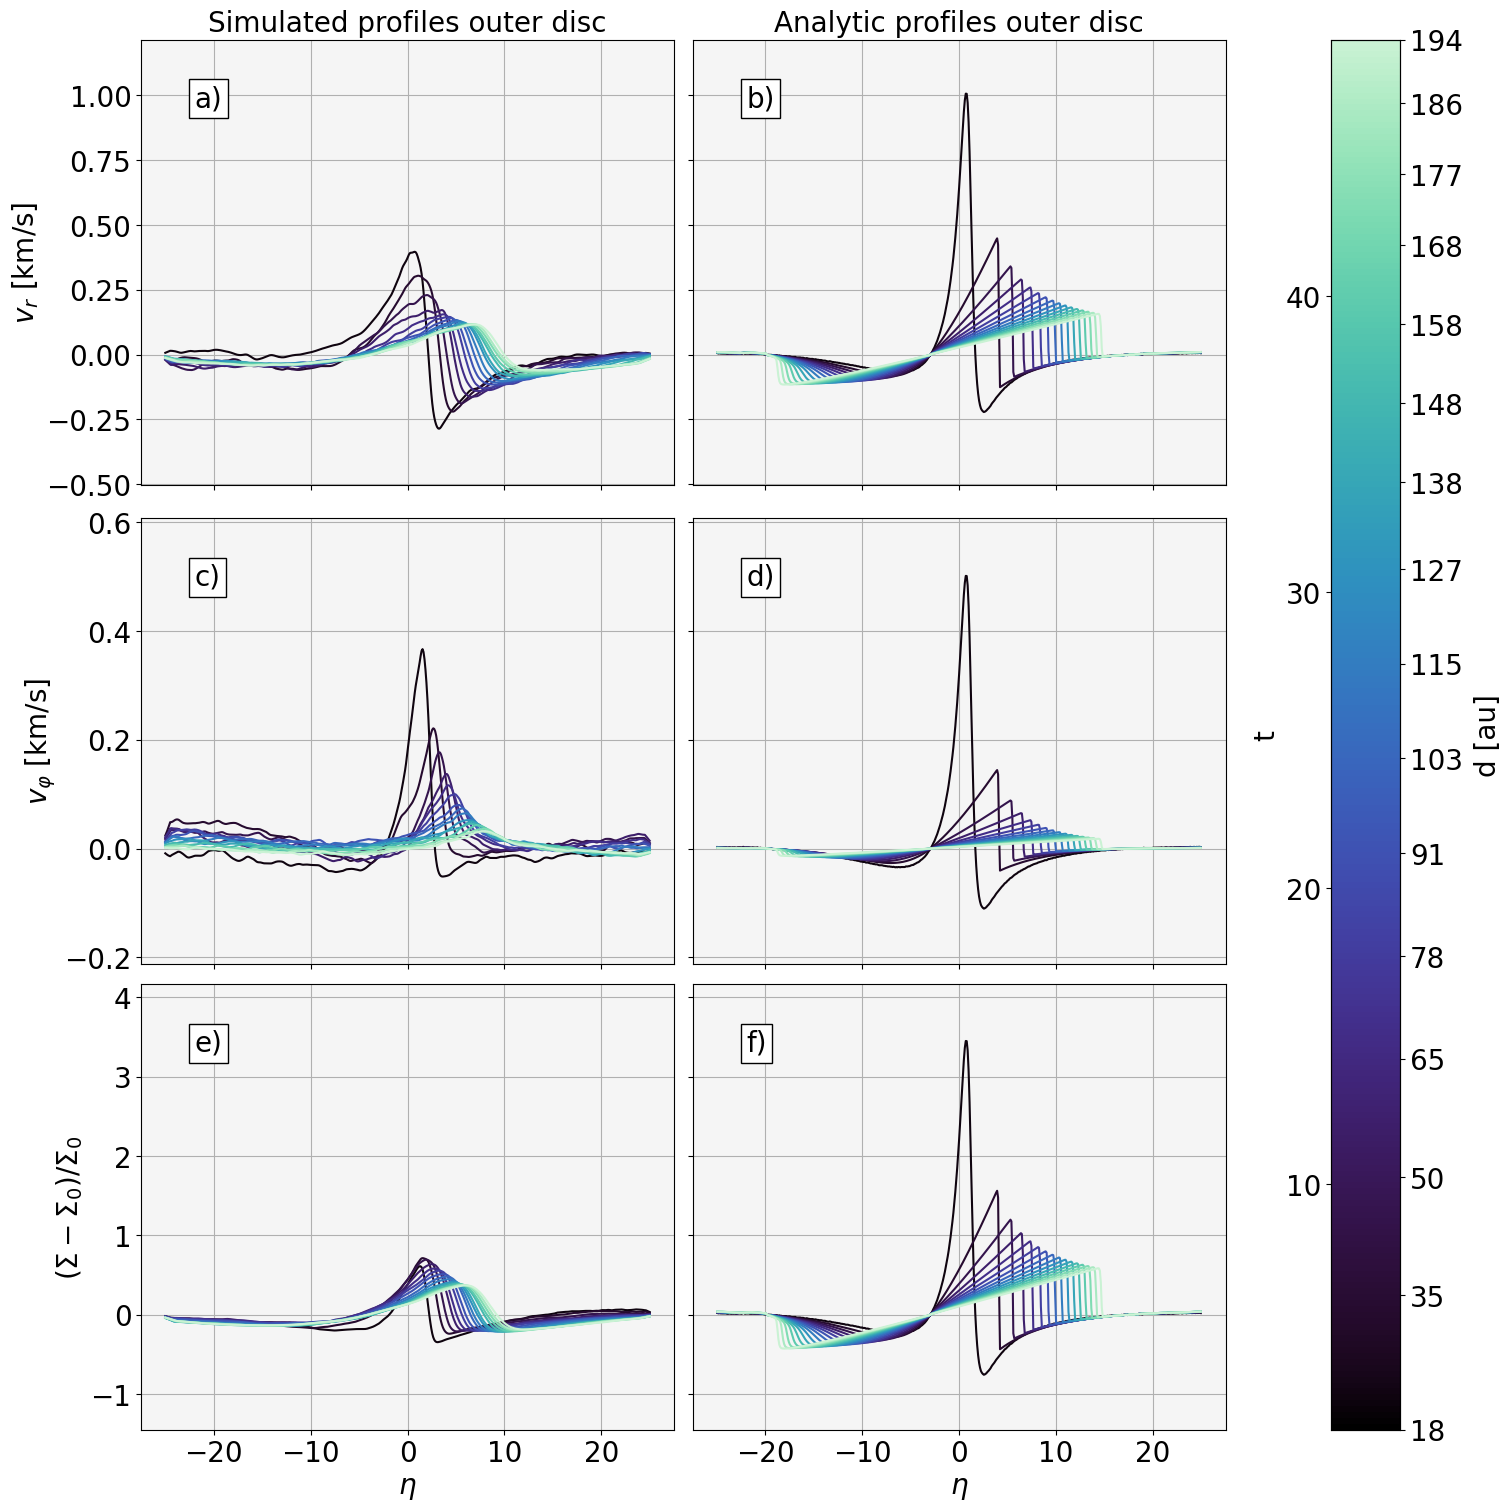
\includegraphics[width = 0.98\textwidth]{figures/comp_as_prof_out_high.png}
    \caption{Comparison between SPH (left) and semi-analytic (right) solutions for the perturbations induced by a $3.87 \, M_{\rm th}$ planet with orbital radius $r_{\rm p}=95.7 \, \mathrm{au}$. Wake profiles taken as slices of constant $t$, or equivalently $r$ are shown. The radial velocity, azimuthal velocity and density perturbations shown from top to bottom. The colourbar indicates the $t$ coordinate for each profile, as well as the physical distance $d$ from the planet location. Figure taken from \citeauthor{fasanoinprep.} (in prep.).}
    \label{fig:profile_comparison}
\end{figure}

However, moving away from the planet and deeper into the non-linear regime the agreement between the analytical and simulated models improves.
Figure \ref{fig:profile_comparison} shows the outer wake profile as it evolves in $t$ for $3.87 \, M_{\rm th}$, compared between both models.
Remarkably, the accuracy in the non-linear regime seems to improve as $t$ increases.
The amplitude for each of the perturbations is in good agreement between the models after the wake was propagated only a few tens of $\mathrm{au}$ from the planet location.
The shocks produced by the inviscid Burger's equation evolution are however steeper than those found in the SPH model, like due to the artificial viscosity present in the simulation \citep{lodato2010}.
The wake profiles are more extended in $\eta$ in the analytics, but we do not seem to recover the over-damping found in the low mass regime by \citet{cimerman2021}.
The position of the outer shock in density, and so the shape of the wake, is also different between the models.
This is not surprising as the pitch angle of the spiral increases and deviates from the linear shape used in the analytics \ref{eq:phi_wake} for high mass planets \cite{zhu2015}.
It may be possible to calibrate for this increase in pitch angle from non-linear effects, see section 5.2 of \citet{cimerman2021} for more details.

The apparent accuracy of the solution in the semi-analytical model far from the planet in the high mass case is perhaps not surprising when considered in the context of the existence of the asymptotic solution given in section \ref{sec:asymptotic_N_wave}.
The more massive planets result in faster shock formation in the Burger's equation evolution, and so it makes at least qualitative sense that the asymptotic solution may also become valid earlier.
The agreement between the analytics and simulations for $t \gtrsim 10$ may therefore reflect that the solution quickly becomes independent of the initial condition, and that the asymptotic scaling in $\chi$ holds well for high planets resulting in the correct non-linear behaviour at some distance from the planet.
We defer further discussions of accuracy, including a full parameter study and a preliminary calibration of the semi-analytic method, to \citeauthor{fasanoinprep.} (in prep.).

\subsection{Velocity Perturbations} \label{sec:velocity_perts}

As we saw in section \ref{sec:nonlinear_evolution} the conservation of the Riemann invariant $R_+$ gives for the radial velocity perturbation
\begin{align}
    u = 2\frac{c_0-c}{\gamma - 1}=-2\frac{c_0}{\gamma + 1} \psi, \label{eq:u_rafikov}
\end{align}
where we define $\psi$ as
\begin{align}
    \psi = \frac{\gamma+1}{\gamma-1} \frac{c - c_0}{c_0},
\end{align}
which is the sound speed perturbation with a constant scale factor. Following \citet{rafikov2002a}, we then derive an expression for $\psi$ in terms of the density perturbation $\chi$ by assuming that the gas obeys a locally polytropic equation of state given by 
\begin{align}
    P = P_0(r) \left[ \frac{\Sigma}{\Sigma_0(r)} \right]^\gamma. \label{eq:poly_EOS}
\end{align}
The sound speed is then
\begin{align}
    c^2 = \frac{\partial P}{\partial \Sigma} = c_0^2(r) \left[ \frac{\Sigma}{\Sigma_0(r)} \right]^{\gamma-1}.
\end{align}
\citet{rafikov2002a} then finds a relation between the density and sound speed perturbations, accurate to second order in $\psi$, found by expanding the above expression. 
This yields
\begin{align}
    \frac{\Sigma - \Sigma_0}{\Sigma_0} = \frac{2}{\gamma + 1}\psi + \frac{3 - \gamma}{\left( \gamma + 1  \right)^2} \psi^2 + \mathcal{O}(\psi^3). \label{eq:psi_exp}
\end{align}
Taking this expression to first order only, we write $u$ in terms of the density perturbation, and then in terms of $\chi$ by substituting equation \ref{eq:chi}. 
\begin{align}
    u = - c_0 \frac{\Sigma - \Sigma_0}{\Sigma_0} = -2 \frac{c_0}{\gamma + 1} \frac{\chi}{g(r)}. \label{eq:ap_rad_vel}
\end{align}
Similarly, \citet{rafikov2002a} finds the azimuthal velocity as
\begin{align}
    v \approx -2 \frac{c_0^2}{\Delta\Omega r} \frac{1}{\gamma + 1} \psi, \label{eq:v_rafikov}
\end{align}
giving to first order in $\psi$
\begin{align}
    v \approx - \frac{c_0^2}{\Delta \Omega r} \frac{\Sigma - \Sigma_0}{\Sigma_0} = - \frac{2}{\gamma + 1} \frac{c_0^2}{\Delta \Omega r} \frac{\chi}{g(r)}. \label{eq:ap_az_vel}
\end{align}
equations \ref{eq:ap_rad_vel} and \ref{eq:ap_az_vel} are the expressions used in \citet{bollati2021} to calculate the velocity perturbations in the non-linear regime. 
Since these are only accurate to first order in $\psi$, the assumption is made that $\psi \ll 1$; indeed \citet{bollati2021} notes that terms proportional to $\psi^2$ are discarded in the derivation of the Burgers evolution \ref{eq:burgers}, and thus also in the calculation of $\chi$ from which $u$ and $v$ are calculated. 
However it is not clear that neglecting the most non-linear terms to calculate the density perturbation $\chi$ necissitates the truncation of the equation of state in the same way. 
Since we are in particular interested in the velocity perturbations, and in planet masses comparable to the thermal mass, we should check if the assumption that $\psi \ll 1$ holds.

We can derive an \textit{exact} expression for $\psi$ in terms of the density perturbation simply by rearranging equation \ref{eq:poly_EOS}. We find
\begin{align}
    \psi = \frac{\gamma + 1}{\gamma - 1} \left[ \left( \frac{\Sigma-\Sigma_0}{\Sigma_0} +1  \right)^{(\psi-1)/2}  -1 \right],
\end{align}
which can be written equivalently in terms of $\chi$ using equation \ref{eq:chi} giving
\begin{align}
    \psi = \frac{\gamma + 1}{\gamma - 1} \left[ \left( \frac{2}{\gamma + 1} \frac{\chi}{g(r)} +1  \right)^{(\psi-1)/2} -1 \right]. \label{eq:psi_exact}
\end{align}
We will use equation \ref{eq:psi_exact} to check the aforementioned assumption that $\psi \ll 1$ in the non-linear regime solution. 
We construct three \textsc{wakeflow} models using dimensionless units, with embedded planet masses of $0.5, 1.0$ and $2.0 \, M_{\rm{th}}$ respectively, all placed in orbit around a $1 \, M_{\rm{\odot}}$ star at an orbital radius of $r=1$. 
For all models, we choose $p=2.25$ and $q=0.25$ such that $\Sigma \propto r^{-1}$, and an aspect ratio $H/r=0.1$ at $r=1$. 
Figure \ref{fig:psi_comparison} shows the values of $\psi$ for each of these models, and demonstrates that even for the lowest planet mass model the value of $\psi$ nearby the planet is as large as $\sim \hspace{-0.23em} 0.6$ and so the second order terms will clearly be important even in this case. 
For masses $\ge \hspace{-0.23em} M_\mathrm{th}$ the problem is even worse, as there are regions where $\psi \gtrsim 1$ causing the expansion given in equation \ref{eq:psi_exp} to diverge.

\begin{figure}
    \centering
    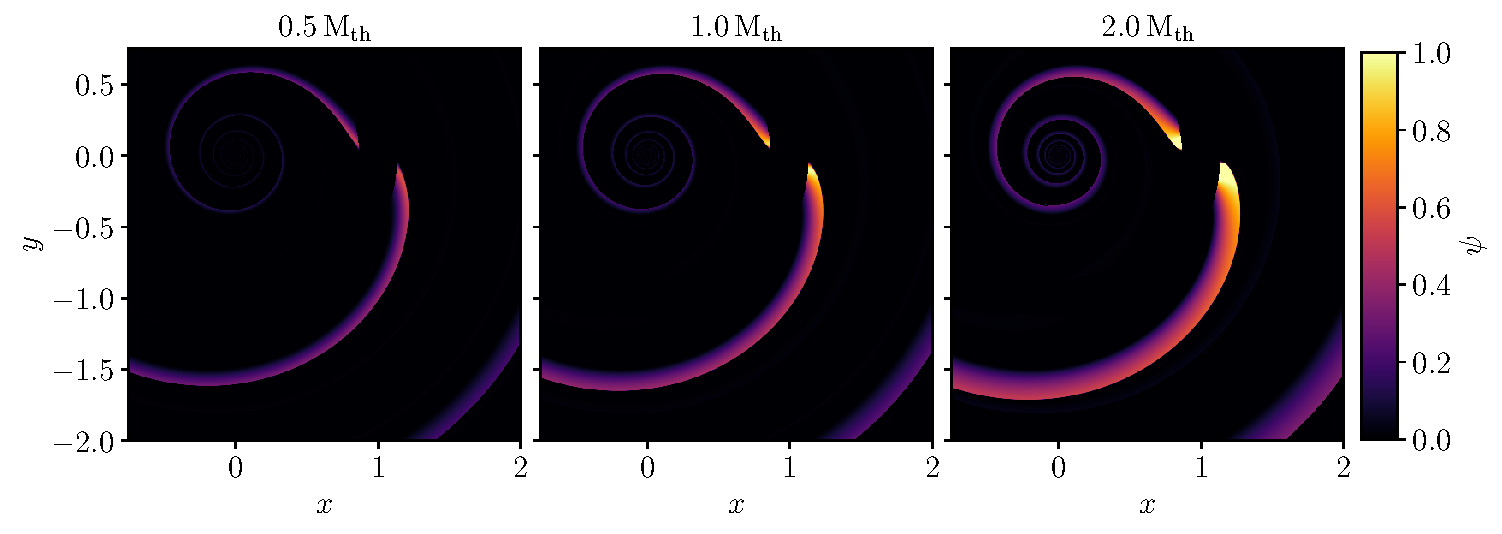
\includegraphics[width = 0.98\textwidth]{figures/psi 2.pdf}
    \caption{Comparison of the values of $\psi$ calculated from equation \ref{eq:psi_exact} for three \textsc{wakeflow} models with planet masses of $0.5, 1.0$ and $2.0 \, M_{\rm{th}}$ respectively. Clearly one cannot assume that $\psi \ll 1$ even for the lowest mass model, especially nearby the planet. For the two larger masses, there are even regions where $\psi > 1$.}
    \label{fig:psi_comparison}
\end{figure}

To improve upon the velocity calculations used in \citet{bollati2021}, here we derive expressions for both $u$ and $v$ as functions of $\chi$ without truncating the equation of state to first order in $\psi$. This is as simple as substituting equation \ref{eq:psi_exact} into equations \ref{eq:u_rafikov} and \ref{eq:v_rafikov}, yielding
\begin{align}
    u(\chi) &= -2 \frac{c_0}{\gamma - 1} \left[ \left( \frac{2}{\gamma + 1} \frac{\chi}{g(r)} +1  \right)^{(\psi-1)/2} -1 \right] \\
    v(\chi) &\approx \frac{c_0}{\Delta\Omega r} u (\chi).
\end{align}




which are the expressions used to calculate the velocity perturbations in the non-linear regime in \textsc{wakeflow}. 

\begin{figure}
    \centering
    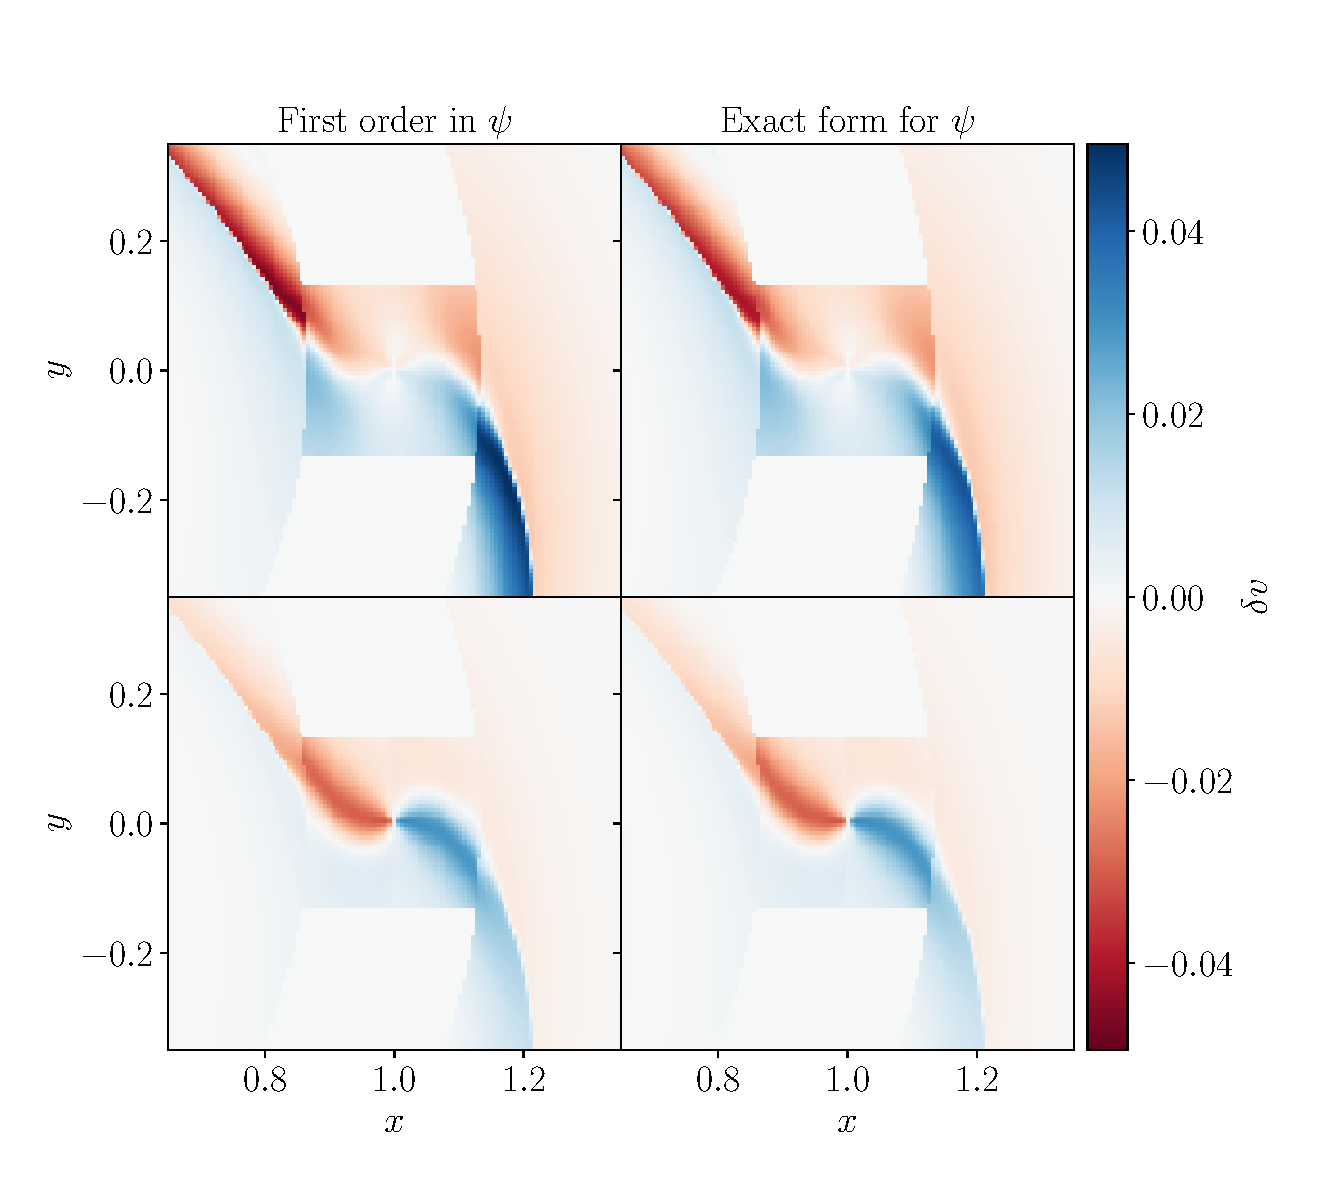
\includegraphics[width = 0.7\textwidth]{figures/0_5_mth.pdf}
    \caption{}
    \label{fig:0_5mth}
\end{figure}

\begin{figure}
    \centering
    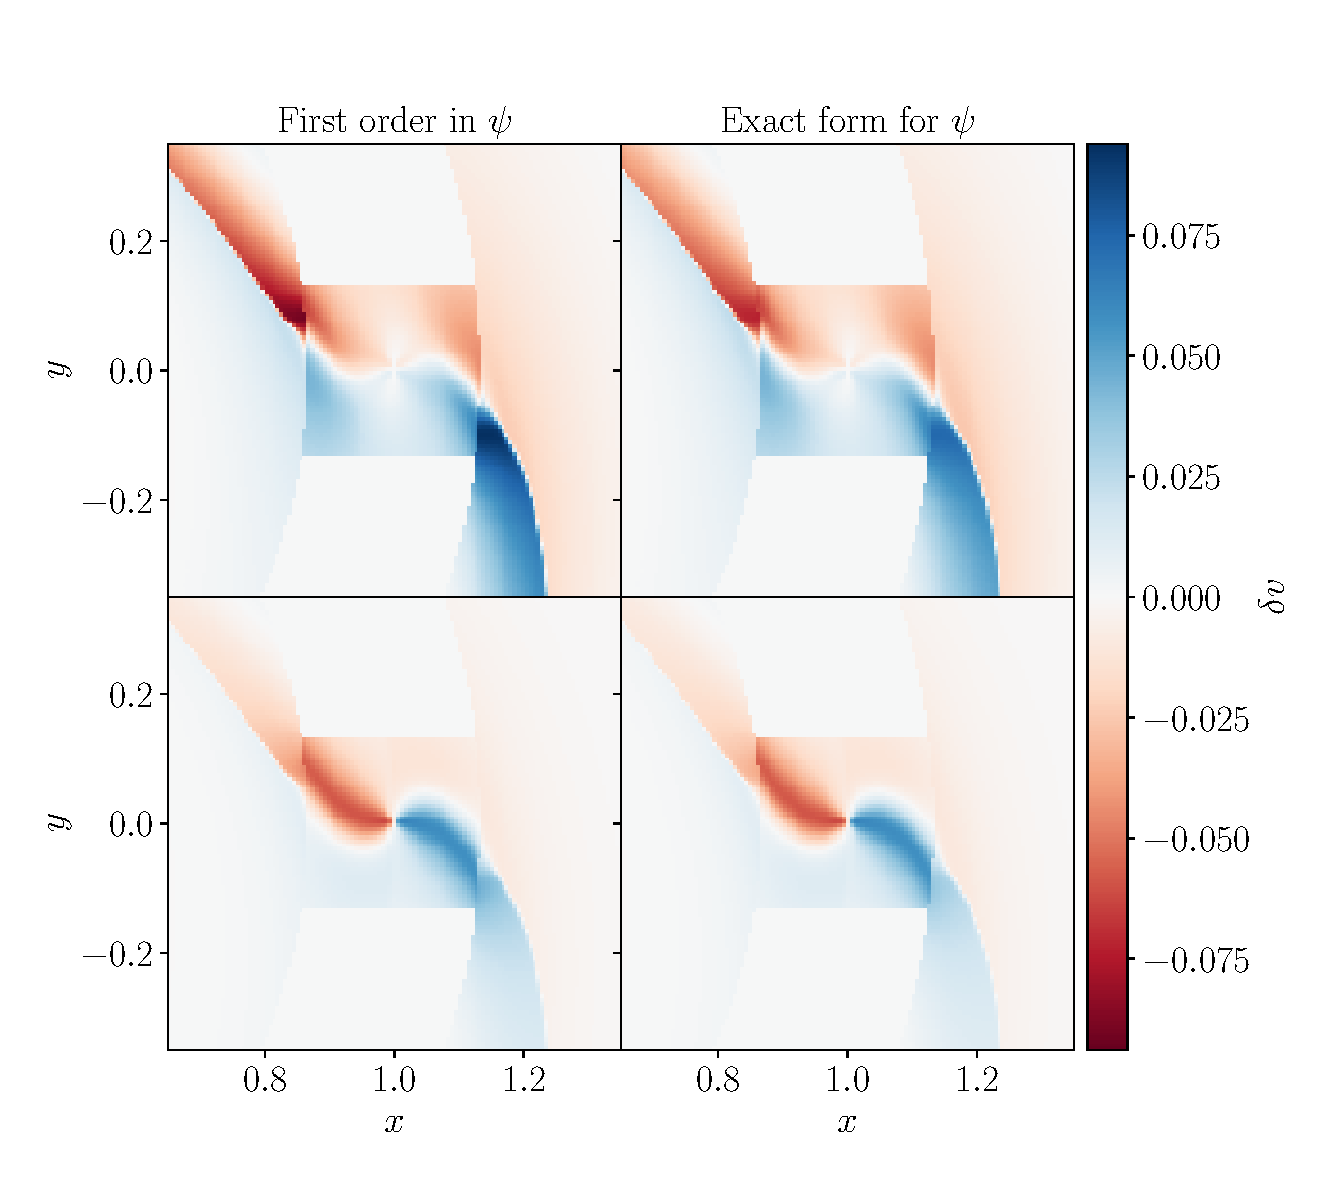
\includegraphics[width = 0.7\textwidth]{figures/1_0_mth.pdf}
    \caption{}
    \label{fig:1_0mth}
\end{figure}

\begin{figure}
    \centering
    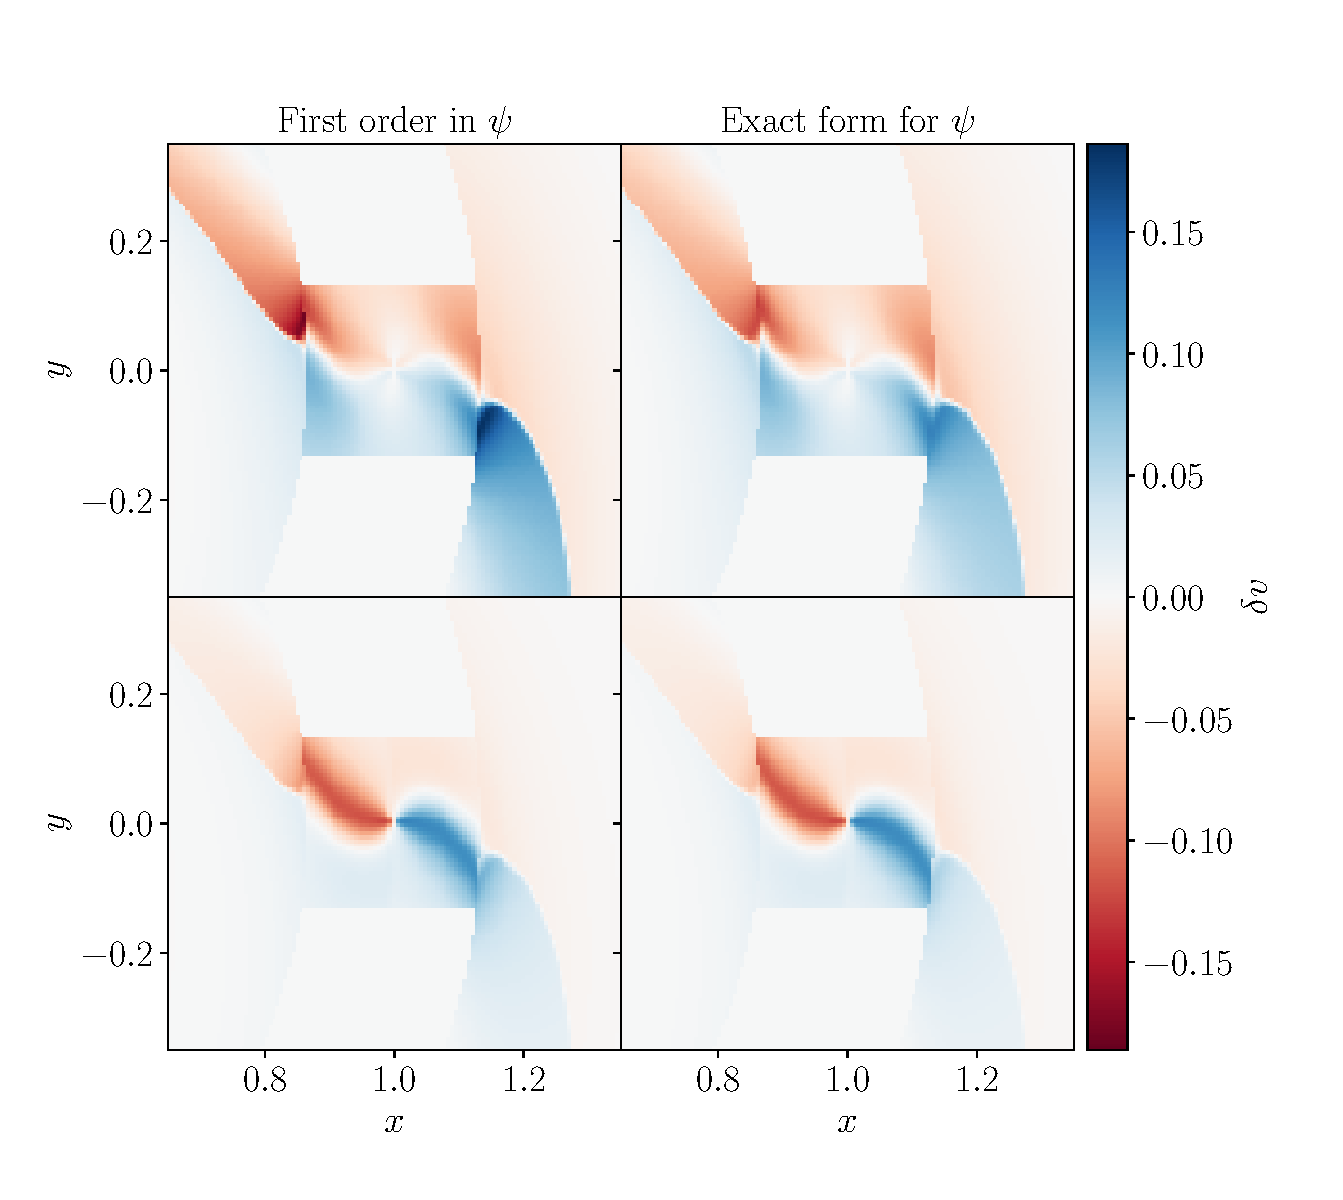
\includegraphics[width = 0.7\textwidth]{figures/2_0_mth.pdf}
    \caption{}
    \label{fig:2_0mth}
\end{figure}



\section{Synthetic Kinematic Observations}

\subsection{Predictions from 2D Models}

\subsection{3D Models}

\subsection{Radiation Transfer}